\section{Analyse}
\subsection{Klassediagram}
Zoals in de bijgevoegde figuur te zien is, hebben we de applicatie opgedeeld in vijf delen:
	\begin{itemize}
		\item de klassen Point, Point3D en Curve; dit zijn ADT's en houden dus specifieke eigenschappen bij en voorzien ook de functies om deze te veranderen. Meer hierover later.
		\item de abstracte klasse Algorithm en zijn subklassen Bezier en Hermite; deze vullen de outputvector van een meegegeven Curve-instantie m.b.v. de input-vector van die instantie. Elk soort algoritme berekent dit anders, uiteraard.
		\item de abstracte klasse Tool en zijn subklassen; deze geven bijvoorbeeld een vector van curves terug indien een afbeelding werd meegegeven, spelen muziektonen af als een vector van curves werd meegegeven,... . Er zijn diverse mogelijkheden en gaandeweg de uitwerking van ons project zal duidelijk worden welke interactiemanier ons het meest optimaal lijkt.
		\item het core-gedeelte: Editor en bijhorende klassen File, Situation en MonitorPool. Editor is het centraal orgaan van de applicatie en stuurt het dataverkeer tussen de verschillende applicatieonderdelen. Situation is een soort van hulpklasse, die bijhoudt welke curve momenteel actief staat, welk type algoritme en welke orde-grootte momenteel aangevinkt staat, welk punt is aangeklikt geweest, \ldots.
 	\end{itemize}


\begin{figure}[hbp]
\center
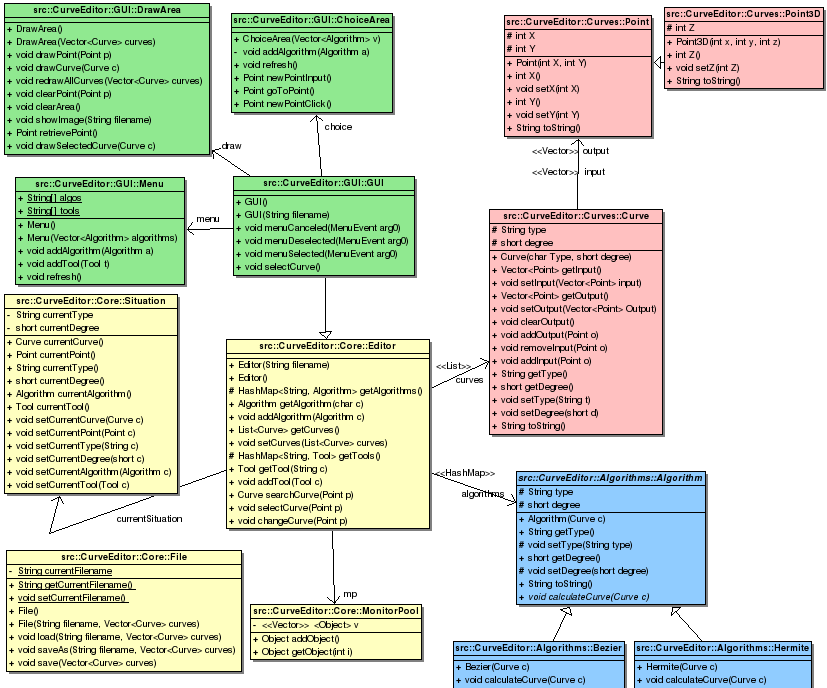
\includegraphics[scale=0.65]{uml.png}
\caption{Het voorlopig UML-diagram.}
\end{figure}
\clearpage

\end{document} 